%% high_throughput_sequencing.tex
%% Author: Leighton Pritchard
%% Copyright: James Hutton Institute
%% These slides briefly introduce the four main sequencing technologies
%% and comment on their relative performance and price.
%% Next they mention Oxford Nanopore as the next promising technology,
%% and the potential impact it could have on sequencing.
%% Finally, the impact that this technology has had on databases and 
%% analyses etc. are described.

% SUBSECTION: Four dominant technologies
% A summary of the characteristics of the four dominant sequencing 
% technologies, and how they can be benchmarked
\subsection{Four dominant technologies}

% The four main current sequencing technologies
\begin{frame}
  \frametitle{Not all sequencing is the same}
  It's all about the biology, but it all starts with the data.\\
  Sequencing technology (including library prep.) affects your sequence data.
  \begin{itemize}
    \item Roche/454 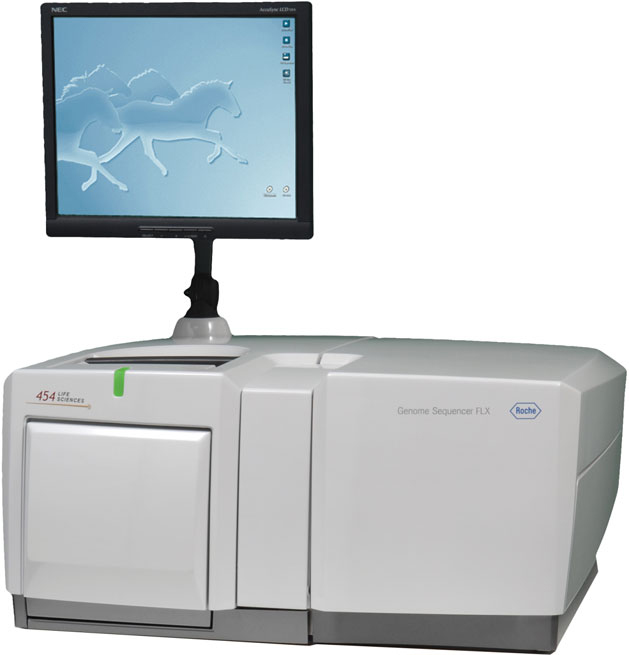
\includegraphics[height=0.15\textheight]{images/454_sequencer}
    \item Illumina 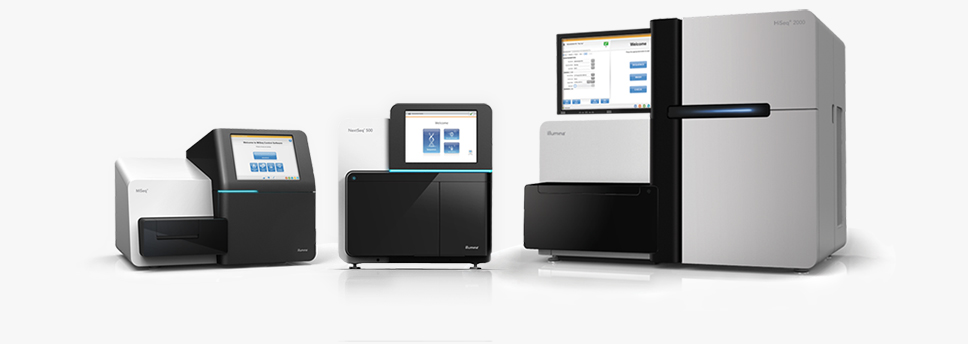
\includegraphics[height=0.15\textheight]{images/miseq_nextseq_hiseq}
    \item Ion Torrent 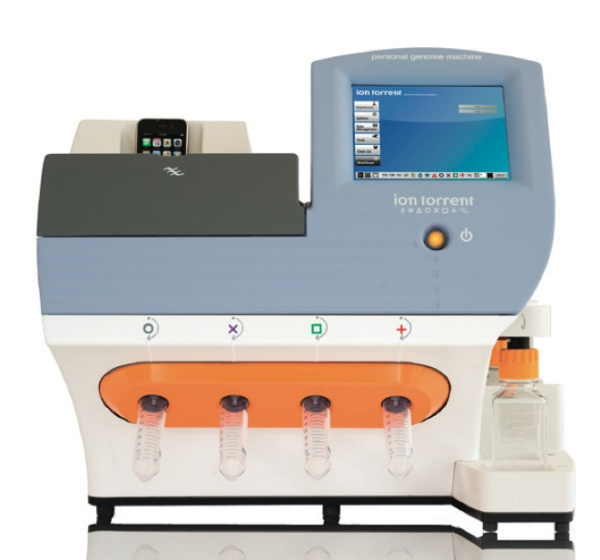
\includegraphics[height=0.15\textheight]{images/ion_torrent_personal_genome_maker}
    \item Pacific Bioscience (PacBio) 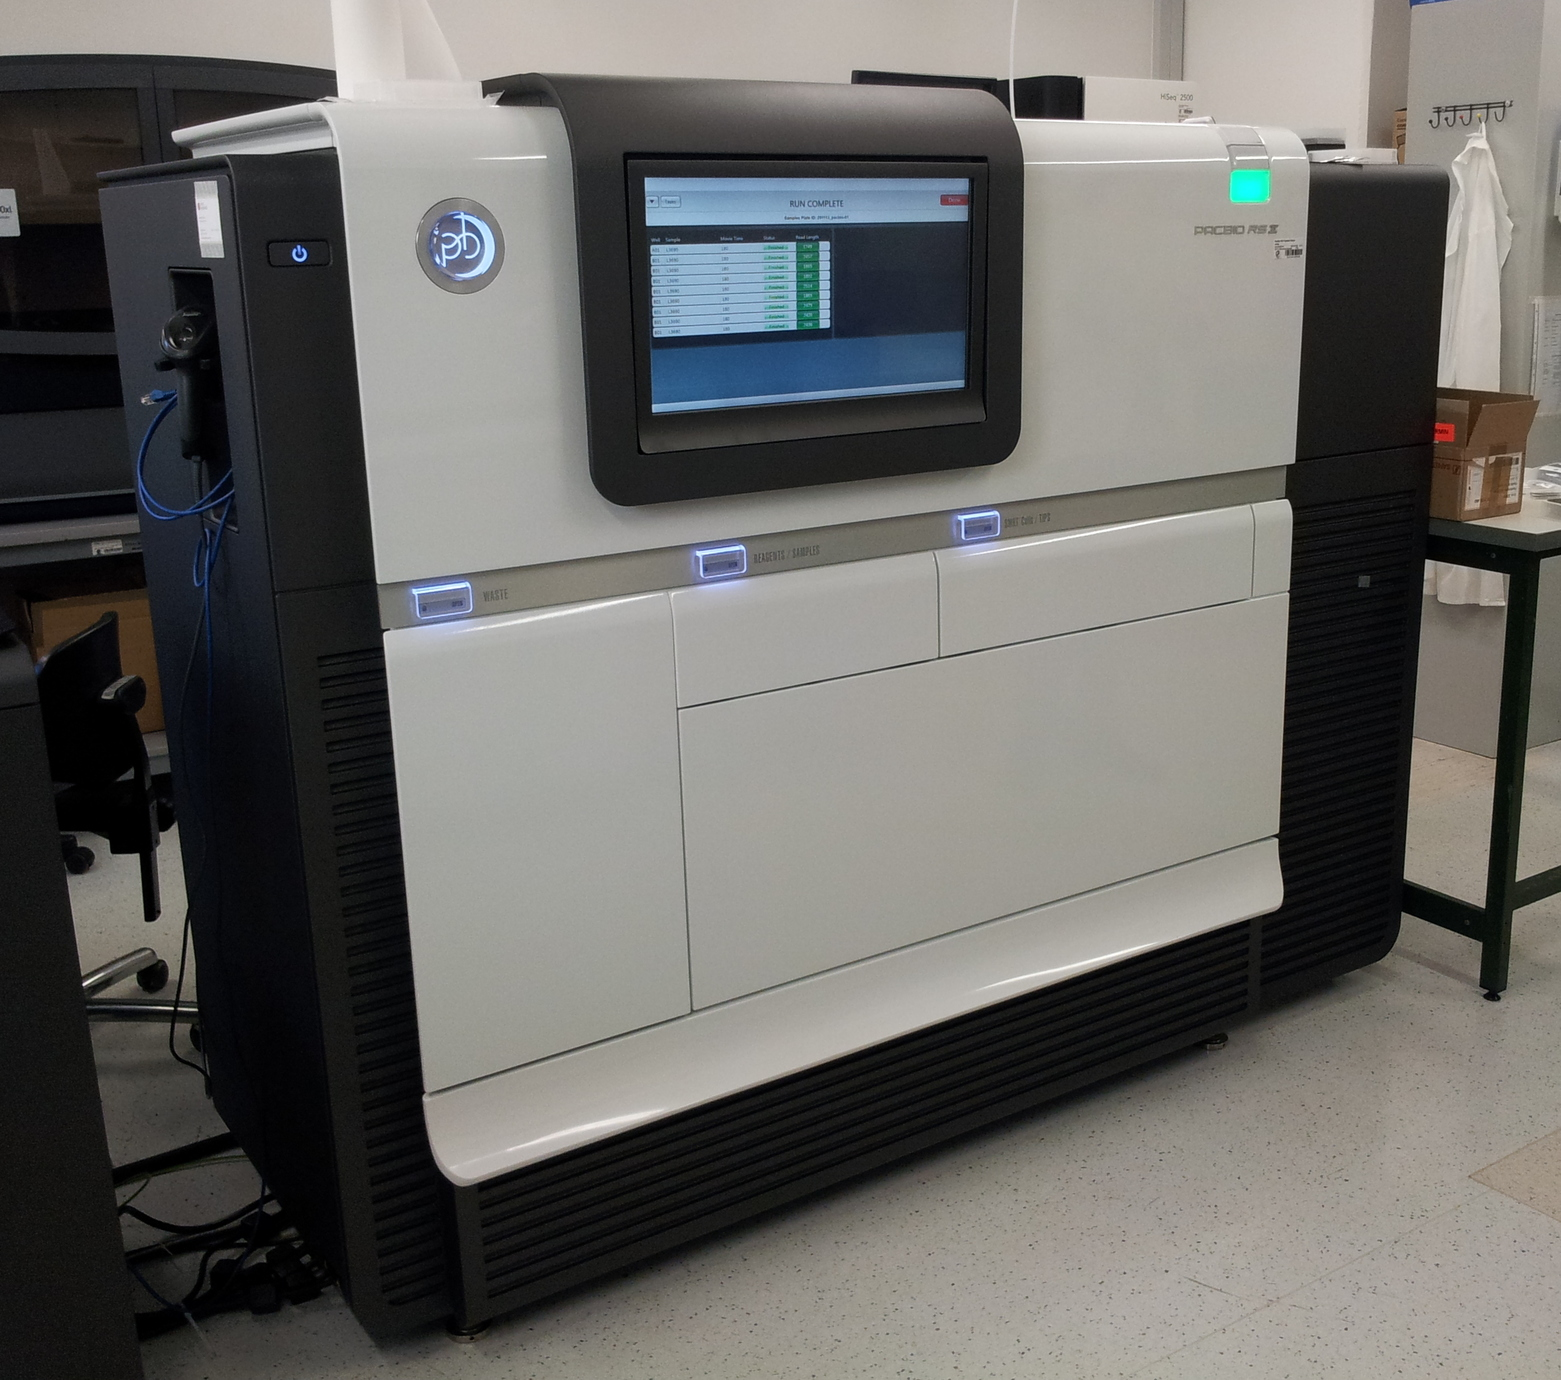
\includegraphics[height=0.15\textheight]{images/PacBio_RSII}
  \end{itemize}
\end{frame}

% Basic principle
\begin{frame}
  \frametitle{The basic principle}
  DNA source is fragmented, and the fragments are sequenced. \\
  \begin{center}
    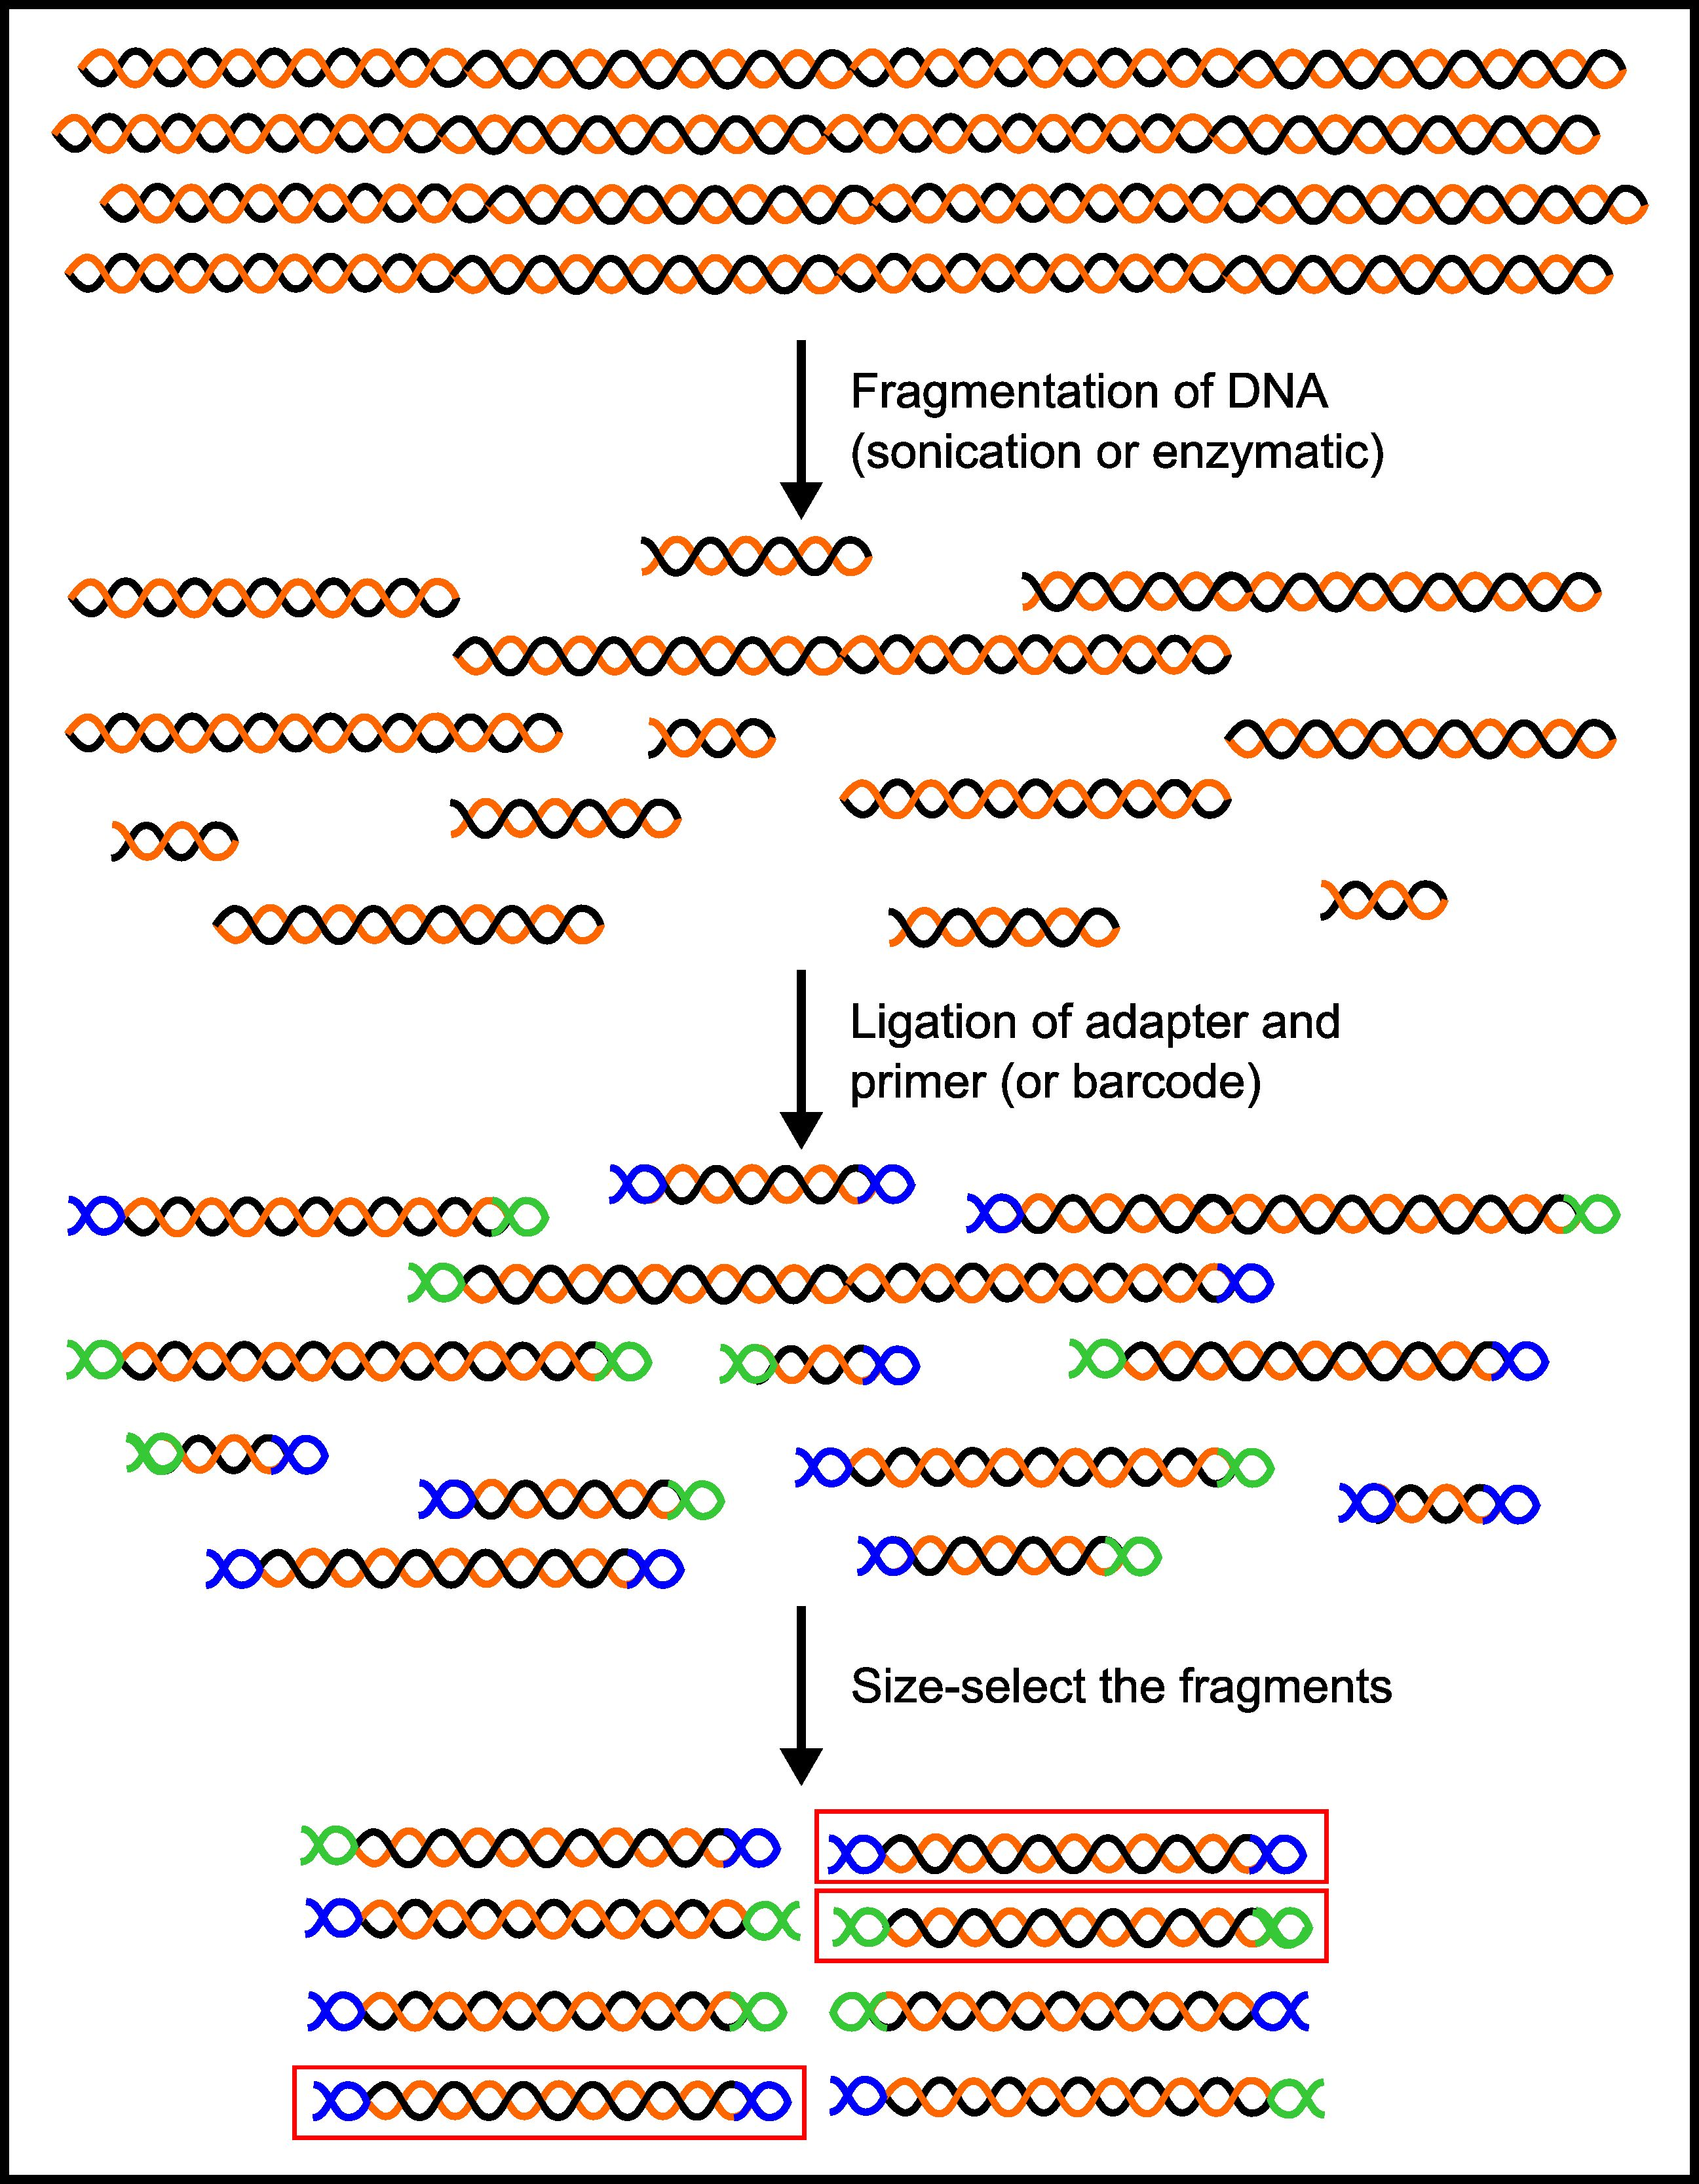
\includegraphics[height=0.7\textheight]{images/library_preparation}
  \end{center}      
\end{frame}

% Paired- and single-end reads
\begin{frame}
  \frametitle{PE vs SE}
  Reads may be single-end, or paired-end.
  \begin{center}
    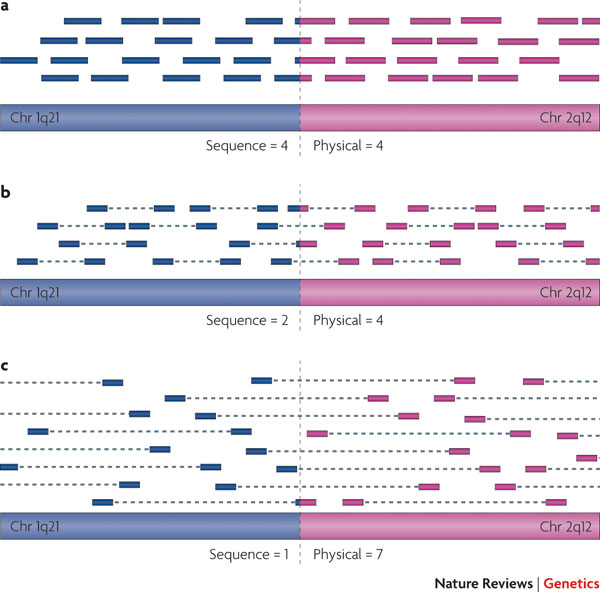
\includegraphics[height=0.6\textheight]{images/pe_vs_se}
  \end{center}      
  Putting the jigsaw back together is sequence assembly.
\end{frame}

% Broad differences in chemistry and output
\begin{frame}
  \frametitle{Four different chemistries\footnote{\tiny{Loman \textit{et al}. (2012) \textit{Nat. Rev. Micro.} \textbf{31}:294-296 \href{http://dx.doi.org/10.1038/nbt.2522}{doi:10.1038/nbt.2522}}}}
  Reads differ by technology, and may require different bioinformatic treatment$\ldots$
  \begin{itemize}
    \item \textbf{Roche/454}: Pyrosequencing (long reads, but expensive, and high homopolymer errors) (700-800bp, 0.7Gbp, 23h)
    \item \textbf{Illumina}: Reversible terminator (cost-effective, massive throughput, but short read lengths) (2x150bp, 1.5Gbp, 27h)
    \item \textbf{Ion Torrent}: Proton detection (short run times, good throughput, high homopolymers errors) (200bp, 1Gbp, 3h)
    \item \textbf{PacBio}: Real-time sequencing (very long reads, high error rate, expensive) (3-15kbp, 3Gbp/day, 20min)
  \end{itemize}
  $\ldots$ different error profiles, varying capability to assemble/determine variation
\end{frame}

% Sequencer relative costs
\begin{frame}
  \frametitle{Costs of sequencing\footnote{\tiny{Miyamoto \textit{et al}. (2014) \textit{BMC Genomics} \textbf{15}:699 \href{http://dx.doi.org/10.1186/1471-2164-15-699}{doi:10.1186/1471-2164-15-699}}}}
    \begin{center}
      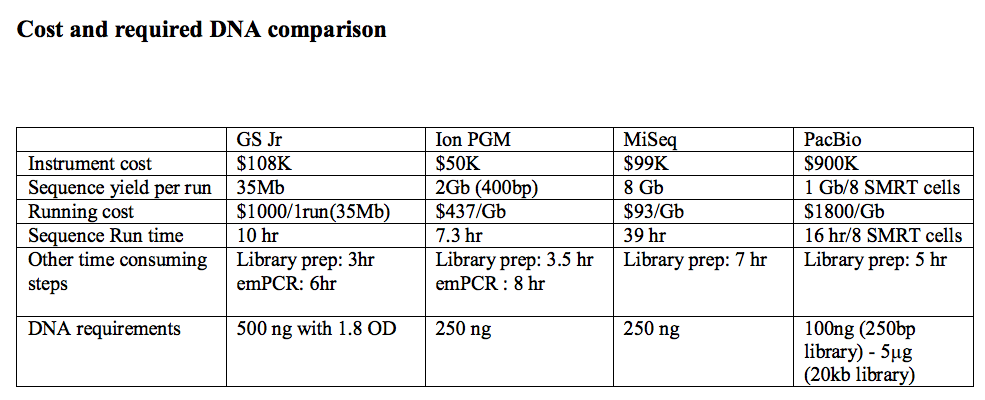
\includegraphics[width=1\textwidth]{images/miyamoto_costs}
    \end{center}      
\end{frame}

% SUBSECTION: Benchmarking
% Summary of benchmarking for sequencing methods: which is best?
\subsection{Benchmarking}

% Benchmarking is very useful
\begin{frame}
  \frametitle{Benchmarked performance}
  Apply several sequencing technologies to the same sample(s). \\  
  Benchmark comparisons inform appropriate choice of sequencing technology%
\footnote{\tiny{Miyamoto \textit{et al}. (2014) \textit{BMC Genomics} \textbf{15}:699 \href{http://dx.doi.org/10.1186/1471-2164-15-699}{doi:10.1186/1471-2164-15-699}}}$^{,}$%
\footnote{\tiny{Salipante \textit{et al}. (2014) \textit{Appl. Environ. Micro.} \textbf{80}:7583-7591 \href{http://dx.doi.org/10.1128/AEM.02206-14}{doi:10.1128/AEM.02206-14}}}$^{,}$%
\footnote{\tiny{Frey \textit{et al}. (2014) \textit{BMC Genomics} \textbf{15}:96 \href{http://dx.doi.org/10.1186/1471-2164-15-96}{doi:10.1186/1471-2164-15-96}}}$^{,}$%
\footnote{\tiny{Koshimizu \textit{et al}. (2013) \textit{PLoS One} \textbf{8}:e74167 \href{http://dx.doi.org/10.1371/journal.pone.0074167}{doi:10.1371/journal.pone.0074167}}}$^{,}$%
\footnote{\tiny{Quail \textit{et al}. (2012) \textit{BMC Genomics} \textbf{13}:341 \href{http://dx.doi.org/10.1186/1471-2164-13-341}{doi:10.1186/1471-2164-13-341}}}$^{,}$%
\footnote{\tiny{Loman \textit{et al}. (2012) \textit{Nat. Biotech.} \textbf{30}:434-439 \href{http://dx.doi.org/10.1038/nbt.2198}{doi:10.1038/nbt.2198}}}$^{,}$%
\footnote{\tiny{Lam \textit{et al}. (2011) \textit{Nat. Biotech.} \textbf{1} (6) \href{http://dx.doi.org/10.1038/nbt.2065}{doi:10.1038/nbt.2065}}} \\[0.5cm]
  Progress in technologies is driving research very rapidly. \\
  Always look for most recent/relevant benchmarks. \\[0.5cm]
  \textbf{Bioinformatic methods also need to be benchmarked.}
\end{frame}

% Benchmarking methods
\begin{frame}
  \frametitle{Benchmarking on \textit{Vibrio}\footnote{\tiny{Miyamoto \textit{et al}. (2014) \textit{BMC Genomics} \textbf{15}:699 \href{http://dx.doi.org/10.1186/1471-2164-15-699}{doi:10.1186/1471-2164-15-699}}}}
    \begin{itemize}
      \item Sequenced \textit{Vibrio parahaemolyticus} (2x chromosomes, closed reference genome) with four technologies
      \item Chose an assembler for each tech, and assembled reads
      \item Excess reads with Ion/MiSeq: used random subsets of reads to determine required coverage 
      \item Aligned assemblies (MUMmer) to known high-quality chromosome sequence, to measure error
    \end{itemize}      
    \begin{center}
      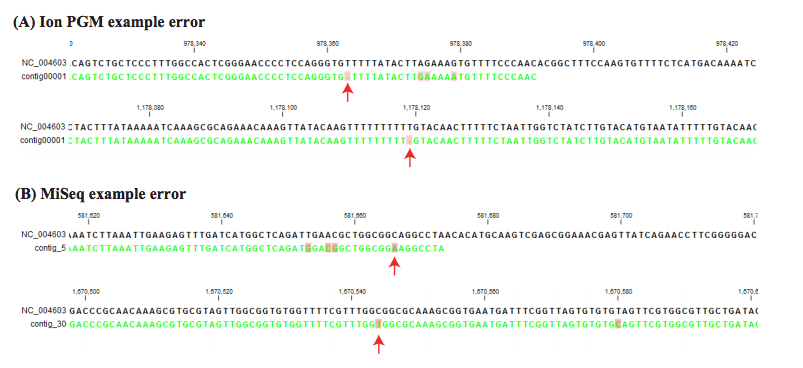
\includegraphics[width=0.8\textwidth]{images/miyamoto_errors}
    \end{center}      
\end{frame}

% Benchmarking results: raw data
\begin{frame}
  \frametitle{Benchmarking on \textit{Vibrio}\footnote{\tiny{Miyamoto \textit{et al}. (2014) \textit{BMC Genomics} \textbf{15}:699 \href{http://dx.doi.org/10.1186/1471-2164-15-699}{doi:10.1186/1471-2164-15-699}}}}
    \begin{center}
      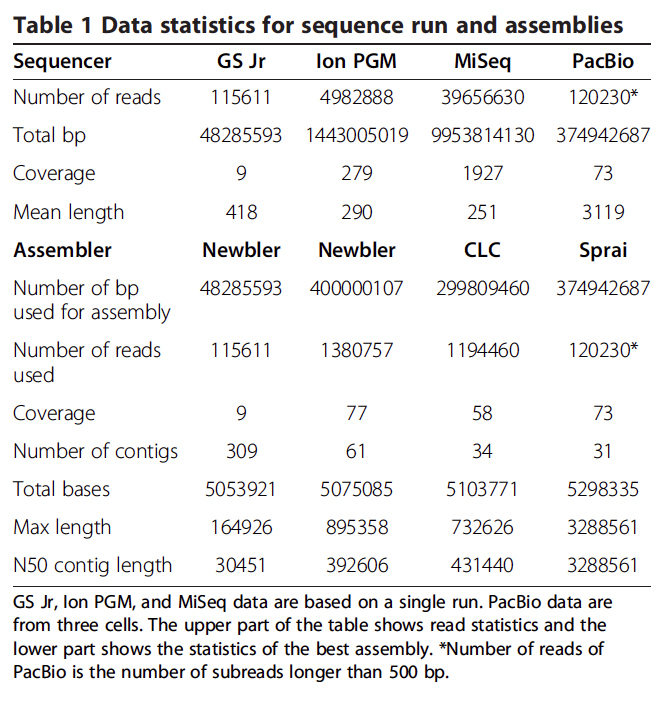
\includegraphics[height=0.8\textheight]{images/miyamoto_table}
    \end{center}      
\end{frame}

% Benchmarking results: alignments
\begin{frame}
  \frametitle{Benchmarking on \textit{Vibrio}\footnote{\tiny{Miyamoto \textit{et al}. (2014) \textit{BMC Genomics} \textbf{15}:699 \href{http://dx.doi.org/10.1186/1471-2164-15-699}{doi:10.1186/1471-2164-15-699}}}}
    \textit{De novo} assembly and alignment against \textit{Vibrio parahaemolyticus} (2x chromosomes)
    \begin{center}
      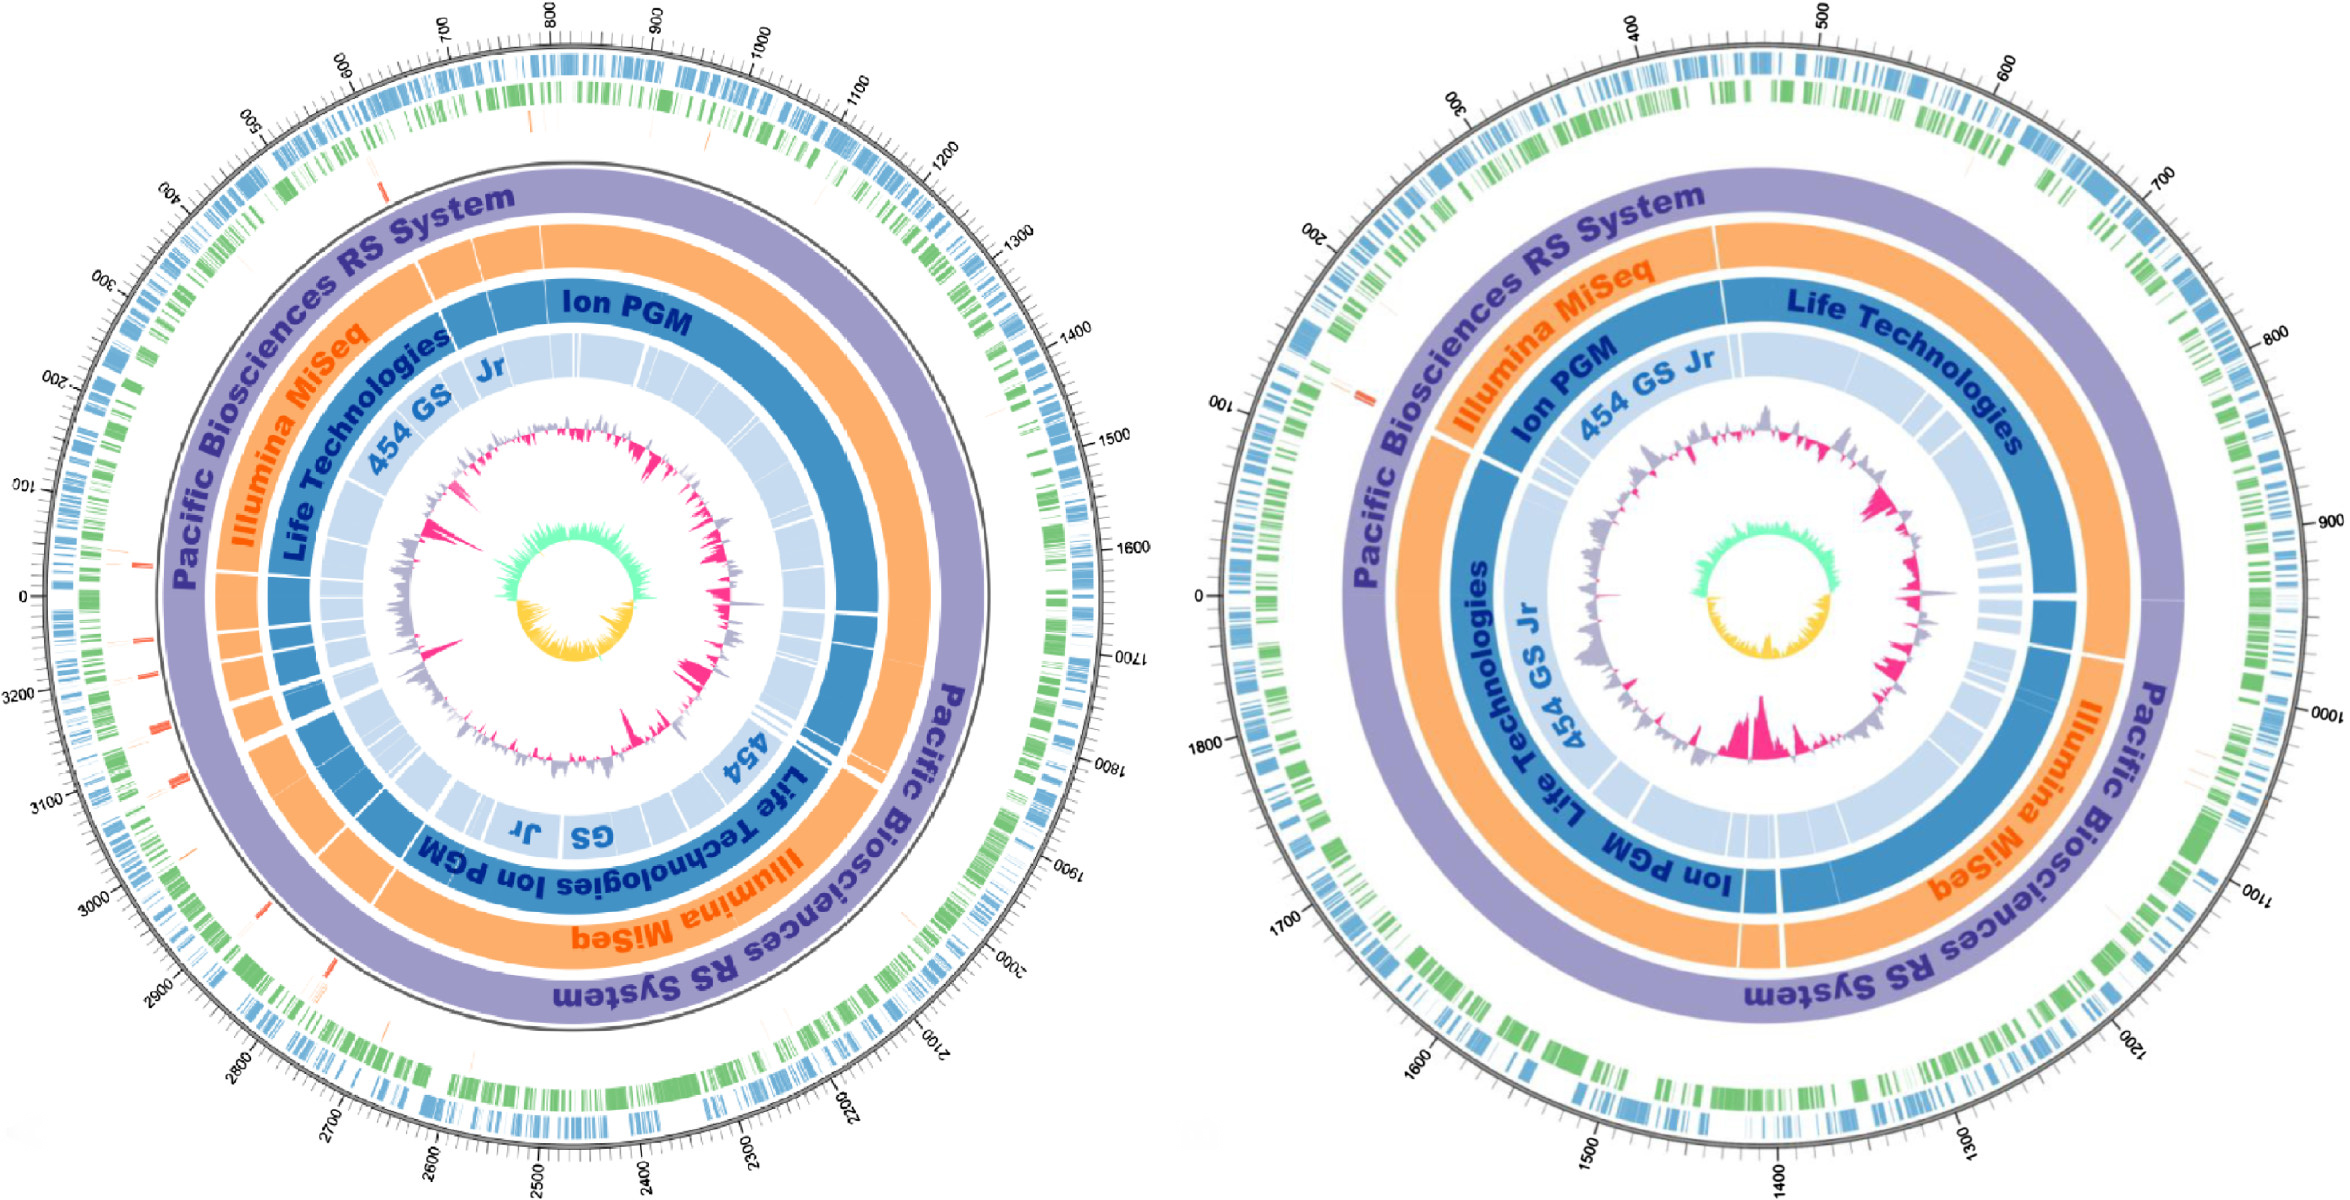
\includegraphics[width=1\textwidth]{images/miyamoto_alignments}
    \end{center}      
\end{frame}

% Benchmarking results: conclusions
\begin{frame}
  \frametitle{Benchmarking on \textit{Vibrio}\footnote{\tiny{Miyamoto \textit{et al}. (2014) \textit{BMC Genomics} \textbf{15}:699 \href{http://dx.doi.org/10.1186/1471-2164-15-699}{doi:10.1186/1471-2164-15-699}}}}
  \begin{itemize}
    \item More and longer reads do not always give the best assemblies: read depth, read distribution, error rate also matters
    \item Optimal assemblies were obtained at around 60x-80x coverage, for Illumina and Ion.
    \item Multiple rRNA regions are fragmented in short-read assemblies
    \item PacBio generated single chromosome contigs
    \item Assembly of multiple-chromosome bacteria is currently feasible
  \end{itemize}  
  Variability in published genomes as methods are not standard (e.g. sequencing technology, assembler, parameter settings and pre-processing)$\ldots$
\end{frame}

% SUBSECTION: Nanopore
% Brief diversion to Oxford Nanopore
\subsection{Nanopore}

% Nanopore
\begin{frame}
  \frametitle{What's just arrived?}
  Oxford Nanopore. A sequencer the size of your hand.
    \begin{center}
      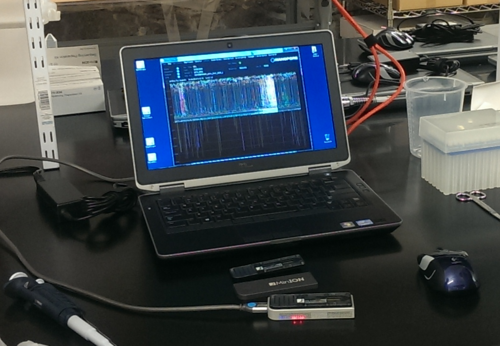
\includegraphics[width=0.48\textwidth]{images/minion_run}\thinspace
      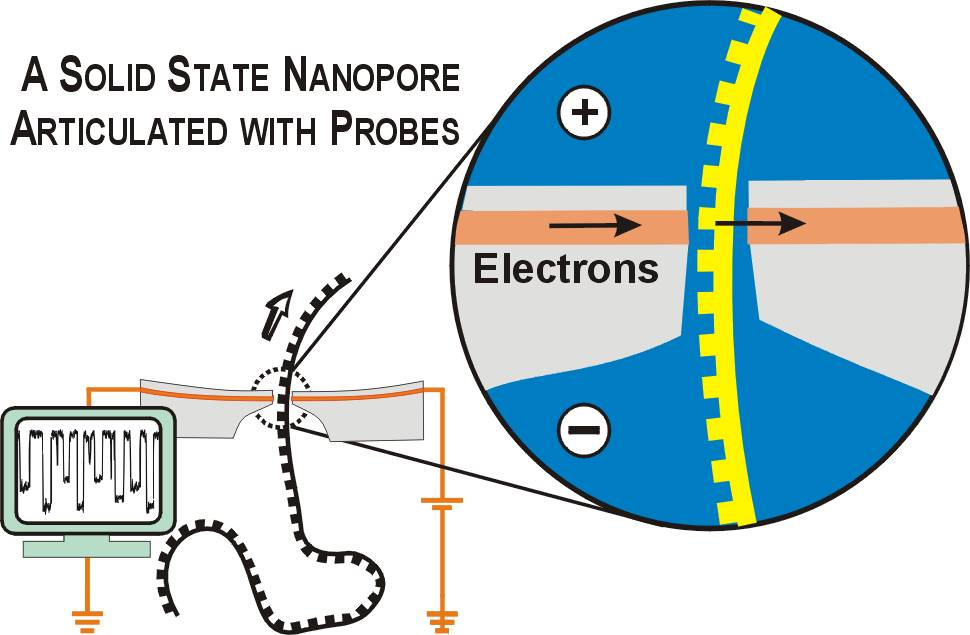
\includegraphics[width=0.48\textwidth]{images/nanopore_schematic}
    \end{center} 
    \begin{itemize}
      \item Microfluidics, single-molecule sequencing; 11-70kbp reads
      \item Reports current across pore (tiny electron microscope) as molecule moves through
      \item \$10/Mbp, 110Mbp per flowcell\footnote{\tiny{Yaniv Erlich (2013) \href{http://erlichya.tumblr.com/post/66376172948/hands-on-experience-with-oxford-nanopore-minion}{Future Continuous blog}}}
    \end{itemize}          
\end{frame}

% Nanopore controversy: paper
\begin{frame}
  \frametitle{Controversy\footnote{\tiny{Mikheyev and Tin (2014) \textit{Mol. Ecol. Res.} \textbf{14}:1097-1102 \href{http://dx.doi.org/10.1111/1755-0998.12324}{doi:10.1111/1755-0998.12324}}}}
  The first Nanopore paper concluded, for $\lambda$ phage:
    \begin{itemize}
      \item About 10\% of reads mapped to the reference genome
      \item \textless1\% of all generated sequence faithfully matches the reference
    \end{itemize}   
    \begin{center}
      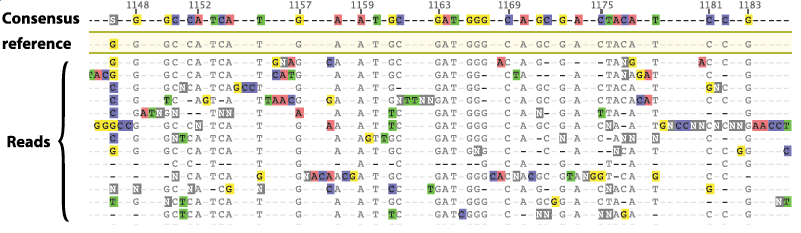
\includegraphics[width=1\textwidth]{images/nanopore_aln}
    \end{center}           
\end{frame}

% Nanopore controversy: response
\begin{frame}
  \frametitle{Controversy\footnote{\tiny{Mikheyev and Tin (2014) \textit{Mol. Ecol. Res.} \textbf{14}:1097-1102 \href{http://dx.doi.org/10.1111/1755-0998.12324}{doi:10.1111/1755-0998.12324}}}}
  Not everyone thinks the Mikheyev and Tin paper is very good:
    \begin{center}
      
\includegraphics[width=0.5\textwidth]{images/nanopore_tweet_1}
      
\includegraphics[width=0.5\textwidth]{images/nanopore_tweet_2}      
    \end{center}           
    \href{http://biomickwatson.wordpress.com/2014/09/07/thoughts-on-oxford-nanopores-minion-mobile-dna-sequencer/}{``But that paper is terrible. It's just lazy.''} (Mick Watson's blog: \href{http://biomickwatson.wordpress.com/2014/09/07/thoughts-on-oxford-nanopores-minion-mobile-dna-sequencer/}{http://biomickwatson.wordpress.com/2014/09/07/thoughts-on-oxford-nanopores-minion-mobile-dna-sequencer/})
\end{frame}

% Some better results
\begin{frame}
  \frametitle{New data\footnote{\tiny{Quick \textit{et al}. (2014) \textit{GigaScience} \textbf{3}:22 \href{http://dx.doi.org/10.1111/1755-0998.12324}{doi:10.1111/1755-0998.12324}}}}
  It's a fast-moving area, and results are improving.
    \begin{center}
      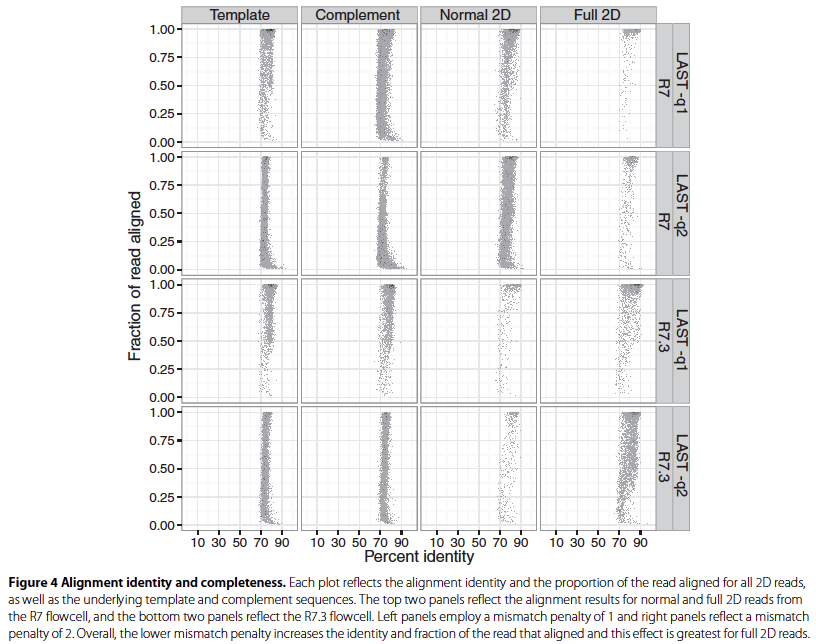
\includegraphics[height=0.65\textheight]{images/nanopore_quick}
    \end{center}           
\end{frame}

% Some better results
\begin{frame}
  \frametitle{New tools}
  Oxford Nanopore's open beta went out without analysis tools.\\
  Tools (Poretools, poRe, etc.) are being written/tested/validated by the user community%
  \footnote{\tiny{Loman and Quinlan (2014) \textit{Bioinformatics} \href{http://dx.doi.org/10.1093/bioinformatics/btu555}{doi:10.1093/bioinformatics/btu555}}}$,$%
  \footnote{\tiny{Watson \textit{et al}. (2014) \textit{Bioinformatics} \href{http://dx.doi.org/10.1093/bioinformatics/btu590}{doi:10.1093/bioinformatics/btu590}}}
    \begin{center}
      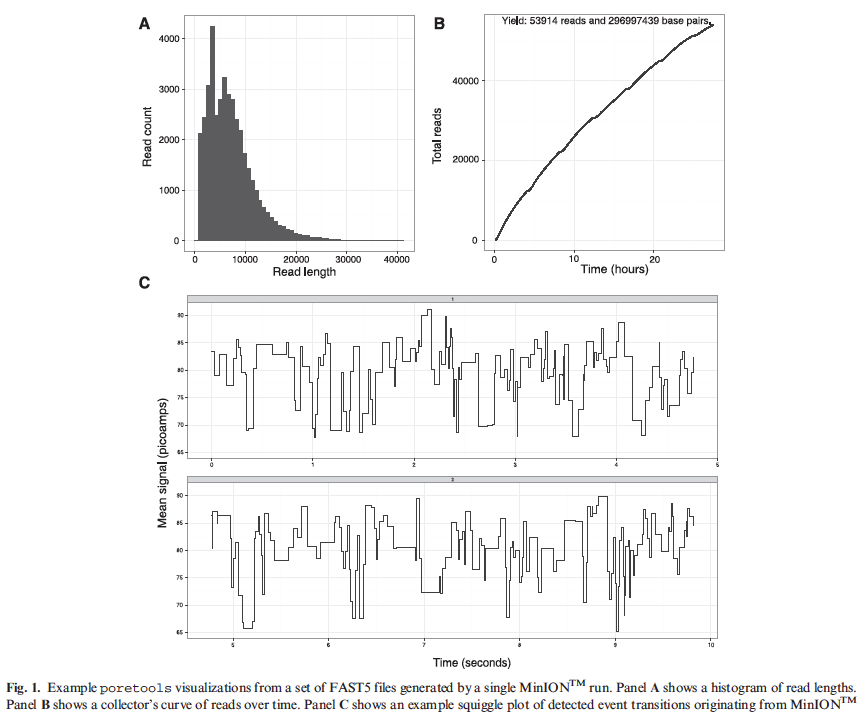
\includegraphics[height=0.55\textheight]{images/poretools}
    \end{center}           
\end{frame}

% SUBSECTION: How fast is data increasing?
% Summary of how fast the amount of sequence data is increasing
\subsection{How fast is sequence data increasing?}

% How many genomes do we have, now?
\begin{frame}
  \frametitle{After that, the flood$\ldots$}
  High-throughput sequencing methods have completely changed the landscape of microbiology \\
  \textbf{(Nearly) complete, (mainly) accurate sequence data is now inexpensive} (and cheaper than analysis)
  \begin{itemize}
    \item \href{http://www.genomesonline.org/cgi-bin/GOLD/index.cgi?page_requested=Complete+Genome+Projects&subset_requested=Complete+And+Published}{GOLD} (19/2/2014): 3,011 ``finished'' ; 9,891 ``permanent draft'' genomes
    \item \href{http://www.genomesonline.org/cgi-bin/GOLD/index.cgi?page_requested=Complete+Genome+Projects&subset_requested=Complete+And+Published}{GOLD} (18/11/2014): 6,649 ``finished'' ; 23,552 ``permanent draft'' genomes    
    \item \href{http://www.ncbi.nlm.nih.gov/Traces/wgs/}{NCBI WGS} (19/2/2014): 17,023 microbial genomes
    \item \href{http://www.ncbi.nlm.nih.gov/Traces/wgs/}{NCBI WGS} (18/11/2014): 26,026 microbial genomes
  \end{itemize}
\end{frame}

% And how many are we going to have?
\begin{frame}
  \frametitle{Predicting the future is hard$\ldots$}
    Su \textit{et al}. attempted to answer this\footnote{\tiny{\href{http://sulab.org/2013/06/sequenced-genomes-per-year/}{http://sulab.org/2013/06/sequenced-genomes-per-year/}}}:
    \begin{center}
      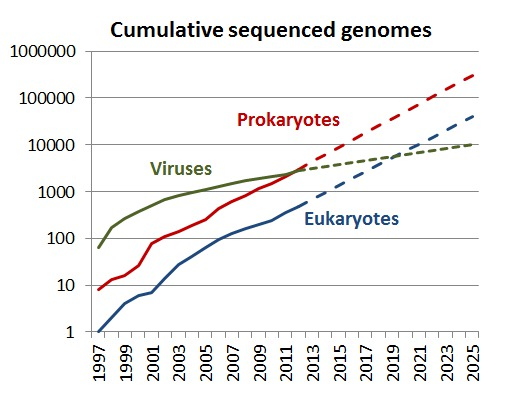
\includegraphics[width=0.5\textwidth]{images/cumulative_sequenced_genomes1}
      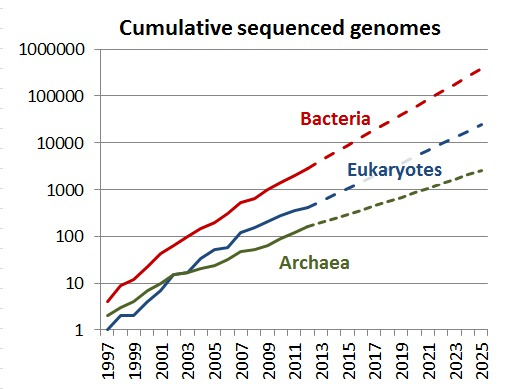
\includegraphics[width=0.5\textwidth]{images/cumulative_sequenced_genomes2}
    \end{center}     
%    How will we keep this much genomic data well-organised?
\end{frame}

% SUBSECTION: Genome sequence standard
% Brief account of MIGS
%\subsection{Genome Sequence and Data Standards}
%
%% MIGS
%\begin{frame}
%  \frametitle{MIGS\footnote{\tiny{Field \textit{et al}. (2008) \textit{Nat. Biotech.} \textbf{26}:541-547 \href{http://dx.doi.org/10.1038/nbt.1823}{doi:10.1038/nbt.1823}}}}
%  Minimum Information about a (Meta)Genome Sequence (MIGS) \\
%  \begin{itemize}
%    \item Standardisation of the data describing a genome sequence; standards are \textbf{essential} to data integrity and reuse
%    \item Defines core descriptors of the data that cannot be derived from the data (geographical context, experimental methods, etc.)
%    \item Produced by \href{http://en.wikipedia.org/wiki/Genomic_Standards_Consortium}{Genomic Standards Consortium} (\href{http://gensc.org/}{gensc.org})
%    \item Provided as checklist and XML schema
%    \item Now also ``Minimum Information about an ENvironmental Sequence'' (MIENS) and others\footnote{\tiny{Yilmaz \textit{et al}. (2011) \textit{Nat. Biotech.} \textbf{29}:541-547 \href{http://dx.doi.org/10.1038/nbt1360}{doi:10.1038/nbt1360}}}
%    \item Global Microbial Identifier (\href{http://www.globalmicrobialidentifier.org/}{http://www.globalmicrobialidentifier.org/})
%  \end{itemize}        
%\end{frame}
%
%% MIGS table
%\begin{frame}
%  \frametitle{MIGS\footnote{\tiny{Field \textit{et al}. (2008) \textit{Nat. Biotech.} \textbf{26}:541-547 \href{http://dx.doi.org/10.1038/nbt.1823}{doi:10.1038/nbt.1823}}}}
%  Minimum Information about a (Meta)Genome Sequence (MIGS) \\
%  \begin{center}
%    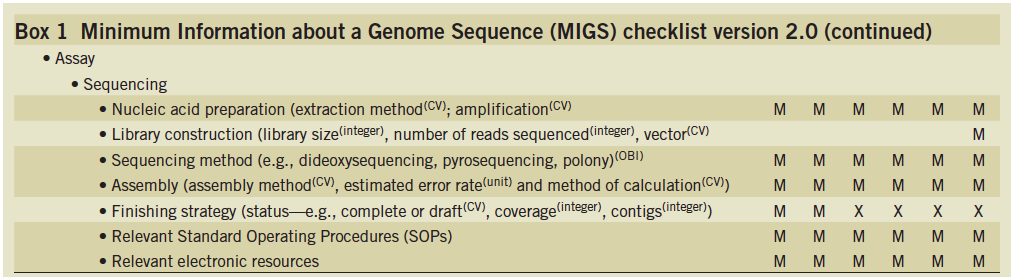
\includegraphics[width=1\textwidth]{images/migs_table}
%  \end{center}           
%\end{frame}